\chapter{Reference Implementation: ExplainableFraud}

\section{Purpose and Scope}
This chapter documents the \emph{ExplainableFraud} companion implementation that instantiates the methodological contracts from Chapter~3 as runnable software. The artefact has two goals: (i) to provide analysts and examiners with a concrete workflow where a transaction feature vector yields a fraud propensity estimate $\hat{y}$, a threshold-based \emph{review} hint, and a structured list of feature-level contributions; (ii) to anchor research questions RQ1--RQ3 in inspectable boundaries---how evaluation metrics and thresholds surface in the UI (RQ1), how explanation narratives are labelled and bounded (RQ2), and how probability-like scores and metadata are wired through versioning and validation artefacts (RQ3).

The implementation is deliberately compact: it targets the public anonymised credit-card benchmark (PCA features \texttt{V1}--\texttt{V28}, \texttt{Time}, \texttt{Amount}) and does not claim parity with industrial rule cascades or multi-hop graphs. Its role in the dissertation is illustrative and reproducible, not a certification of production readiness.

From a scholarly standpoint, the artefact constitutes an \emph{instrument} that makes Chapter~3's contracts observable: thresholds materialise as UI affordances rather than latent configuration; explanation methods acquire explicit textual labels beside numeric decompositions; and model lineage appears as immutable-looking strings surfaced to the examiner. Throughout this chapter, occurrences of ``probability'' denote the scorer's numerical output interval $[0,1]$ plus whatever calibration metadata accompanies the trained pipeline—they should not be read as audited long-run frequencies unless corroborated by offline reliability studies in Chapter~5.

\subsection*{Traceability map for RQ1--RQ3}
Table~\ref{tab:rq-ui-traceability} summarises where each research question leaves a visible footprint in the running system. Readers may treat it as an index tying narrative claims to inspectable artefacts; citations point to the argumentative spine in Chapters~2--3 rather than to UI strings.

\begin{table}[htbp]
\centering
{\footnotesize\setlength{\tabcolsep}{4pt}\renewcommand{\arraystretch}{1.08}%
\resizebox{\linewidth}{!}{%
\begin{tabular}{p{2.1cm}p{6.2cm}p{6.35cm}}
\toprule
\textbf{RQ} & \textbf{Theoretical anchor (Chs.~2--3)} & \textbf{Examiner-visible surface} \\
\midrule
RQ1 & PR-centric evaluation under rarity; threshold policies \cite{davis_goadrich_icml06,fraud_handbook}. & Threshold $\tau$, Boolean review hint triggered when $\hat{y}\geq\tau$, optional validation metrics card wired to exported evaluation JSON. \\
RQ2 & Post-hoc attributions as bounded sensitivity summaries, not causal proofs \cite{xai_survey}. & Declared explanation method label, ranked normalised contributions, adjacent narrative caveats discouraging causal reading. \\
RQ3 & Calibration and lineage discipline when scores read as probabilities \cite{niculescu_caruana_calib2005}. & Model or version identifiers, heuristic fallback when artefacts are missing, deterministic JSON payloads for scripted replay. \\
\bottomrule
\end{tabular}}}
\caption{Research questions (RQ1--RQ3) mapped to examiner-visible surfaces.}
\label{tab:rq-ui-traceability}
\end{table}

\section{Operational guide for analysts and reviewers}
\label{sec:operational-guide}
This section adopts the perspective of a human operator who encounters the artefact cold and must progress from idle processes to defensible interpretations. Institutional pilots would expand each step with access control runbooks and ticket integration; here the emphasis remains academic reproducibility coupled with behavioural clarity.

\subsection{Topology and prerequisites}
Three cooperating responsibilities underpin the demonstration: an ASP.NET Core API hosting synchronous fraud scoring (\texttt{/api/\allowbreak fraud/\allowbreak score}), ancillary asynchronous training simulations (\texttt{/api/\allowbreak training/...}), and Swagger documentation exposing both controllers; concurrently, the Blazor Server site supplies the transactional form (\texttt{/fraud}) plus the experimentation dashboard (\texttt{/training}). Separate typed \texttt{HttpClient} registrations obtain \texttt{ApiBaseUrl} from configuration; if the UI cannot reach the API, users observe transport-level errors rather than silent score substitution or mocked metrics. Screenshots referenced later assume both hosts run with bundled HTTP launch profiles (\texttt{Explainable\allowbreak Fraud.Api}, \texttt{Explainable\allowbreak Fraud.Web}) and that firewall rules permit loopback connections.

\subsection{Step-by-step walkthrough}
Figure~\ref{fig:ui-fraud-form} complements the enumerated procedure below.

\begin{enumerate}
    \item \textbf{Bootstrap services.} Start the API (ML pipeline zip reachable per configuration); start the web project; verify Swagger lists \texttt{POST /api/\allowbreak Fraud/\allowbreak score}.
    \item \textbf{Confirm connectivity settings.} The web host reads \texttt{ApiBaseUrl} (representative developer value \url{http://localhost:5039/}). Misaligned bases yield failed POST attempts before any model logic executes.
    \item \textbf{Enter transaction primitives.} On \texttt{/fraud}, supply monetary \texttt{Amount} using the corpus units (non-negative decimals), \texttt{Time} elapsed in seconds measured compatibly with the public dataset's temporal column semantics, and—if exercised—comma-separated PCA coordinates spanning \texttt{V1} through \texttt{V28}. Empty advanced vectors default to zeros, reproducing padded inputs expected by the bundled trainer pipeline.
    \item \textbf{Submit for scoring.} The form emits \texttt{Fraud\allowbreak Score\allowbreak Request} JSON to \texttt{POST /api/fraud/\allowbreak score}. Validation rejects oversized PCA lists to prevent silent truncation bugs.
    \item \textbf{Read decision support artefacts.} The response hydrates dashboard cards: probabilistic $\hat{y}$, configured $\tau$, model identifier, explanations, optional validation metrics when ancillary JSON ships with artefacts.
    \item \textbf{Optional visual analytics.} The \texttt{/visuals} route hosts charts suitable for pedagogical exposition; scoring logic remains unaffected.
    \item \textbf{Optional training experimentation.} The \texttt{/training} dashboard (documented systematically in Section~\ref{sec:training-surface}) exercises catalogued datasets and ML.NET families under explicit simulation controls; defer to that section before mixing UI numbers with archival CLI exports.
\end{enumerate}

\subsection{Semantics of assembled inputs}
\noindent
Although anonymised PCA dimensions lack merchant-specific lexicons, they still induce a well-defined predictor domain once training commits a scaling policy. Analysts should interpret each field as follows:

\smallskip
\noindent
\begin{tabularx}{\textwidth}{@{}l X@{}}
\toprule
\textbf{Field} & \textbf{Operational reading (demonstration scope)} \\
\midrule
\texttt{Amount} & Scalar transaction magnitude; influences scale-sensitive tree splits and deviates relative to training moments in explanation weighting. \\
\texttt{Time} & Relative seconds feature mirroring the published benchmark; drift relative to training distribution can inflate z-style deviation terms. \\
\texttt{V1}--\texttt{V28} & Orthogonalised coordinates encoding latent structure; absent coordinates default to PCA-space padding only if training mirrored the same convention. \\
\bottomrule
\end{tabularx}

\subsection{Interpreting the fraud score and review threshold}
The primary scalar output is a fraud propensity estimate $\hat{y}\in[0,1]$ produced by \texttt{Prediction\allowbreak Engine} when a serialised ML.NET model is present. The UI compares $\hat{y}$ with a deployment threshold $\tau$ exported alongside the pipeline; crossing the threshold toggles a Boolean review flag intended for triage queues. This construction instantiates RQ1 operationally: instead of discussing threshold policies abstractly, the artefact forces the observer to confront a single committed $\tau$ while keeping open the possibility of contrasting alternative policies through exported validation metrics. When scores behave as ranking surrogates only, interpret $\hat{y}$ ordinally; when calibration artefacts exist, align verbal probability statements with empirical frequency checks from Chapter~5.

\subsection{Interpreting contributions and method tags}
Explanations appear as normalised non-negative contributions summing to unity after post-processing, ordered for rapid scanning. Each list carries a method identifier (\texttt{Metadata\allowbreak Weighted\allowbreak Deviation} in the reference build) clarifying that values arise from a hybrid of global importance weights and per-feature z-scores—not from Shapley efficiency nor LIME surrogate coefficients. This addresses RQ2 by making epistemic status visible: analysts can sort features to prioritise manual checks yet must not treat ranks as causal attributions or legal evidence of intent. Short textual summaries adjacent to the chart restate the same caveats to reduce the risk of dashboard misreading during live demos.

\subsection{Limitations explicit in the reference build}
The companion software omits multi-tenant authentication, streaming ingestion, graph enrichment, behavioural sequences, investigator feedback capture, chargeback reconciliation, and live retraining—all standard in regulated payment stacks \cite{fraud_handbook,lucas_jurgovsky_ccfraud_survey2020}. Explanation stability across adversarial perturbations is not monitored; heuristic scoring activates when artefacts are absent, signalling engineering resilience but offering no calibrated fraud probability. Readers should weigh these omissions when mapping the dissertation narrative onto prospective industrial pilots.

\section{Model training experimentation surface}
\label{sec:training-surface}

The artefact exposes an additional analyst-facing route (\texttt{/training}) devoted to reproducible ML.NET experimentation without requiring external notebooks whenever the API simulation layer is enabled (see \texttt{TrainingJobs:\allowbreak Simulation} in repository settings). The Blazor Server page retrieves dataset catalogue metadata via \texttt{GET /api/\allowbreak training/\allowbreak datasets}, starts asynchronous jobs (\texttt{POST /api/\allowbreak training/\allowbreak jobs}), and polls job status endpoints (\texttt{GET /api/\allowbreak training/\allowbreak jobs/}, then a GUID suffix) until termination. Transparency covers data provenance (offline CSV versus seeded synthetics), trainer lineage, staged execution, evaluator summaries, coarse wall-clock duration, badges announcing synthetic versus observational sources, contextual footers distinguishing timeline-only mocks from genuine estimator runs, complementing the operational scoring prerequisites from Section~\ref{sec:operational-guide}.

\subsection{Analyst-facing walkthrough on \texttt{/training}}
Enumerate the workflow below beside Section~\ref{sec:operational-guide}.
\begin{enumerate}
    \item \textbf{Booth API and Web together.} Interactive training executes inside \texttt{Explainable\allowbreak Fraud.Api}; Razor merely polls JSON snapshots. Align \texttt{ApiBaseUrl} exactly as during fraud scoring demos.
    \item \textbf{Confirm simulation semantics.} Setting \texttt{UseSimulation} to \texttt{false} beneath \texttt{TrainingJobs:\allowbreak Simulation} rejects job enqueueing until operators re-enable the mock orchestrator\textemdash guarding restricted notebook shells. Turning \texttt{RunSynthetic\allowbreak InProcessTraining} off deliberately exercises \emph{timeline-only} progress without invoking \texttt{Fit}; explanatory copy warns reviewers that metrics collapse into placeholders unless the truthful evaluator path stays enabled.
    \item \textbf{Select dataset lineage.} Two catalogue entries advertise ULB/\allowbreak Kaggle-style semantics (\texttt{Time}, \texttt{V1}--\texttt{V28}, \texttt{Amount}, \texttt{Class}). Their textual descriptions differ principally in deterministic synthetic multiplicity when CSV discovery misses\textemdash \texttt{Creditcard\allowbreak LocalCsv} multiplies configurable synthetic targets versus the sibling label.
    \item \textbf{Offline CSV ingestion or synthetic fallback.} Configurable relative-path probes resolve \texttt{creditcard.csv} underneath the API content root or alternate approved folders; ingestion requires no outbound network hops. Canonical public releases contain about $284\,807$ rows \cite{credit_card_dataset}, mirrored heuristically in configuration commentary (\texttt{Reference\allowbreak Kaggle\allowbreak Cardinality}) and truncated only via explicit row caps (\texttt{MaxCreditcardCsv\allowbreak RowsToLoad}). Absent compliant files the service fabricates deterministic ULB-shaped rows whose minimum floor respects at least ten thousand transactions (\texttt{MinSyntheticTraining\allowbreak RowCount}), guarding classroom stability alongside tunable imbalance fractions.
    \item \textbf{Trainer families versus neural placeholder.} The picker surfaces logistic LBFGS baselines (\texttt{L-BFGS} via ML.NET logistic regression trainers), boosted decision trees (\texttt{FastTree}), bagged ensembles (\texttt{FastForest}), and an \emph{experimental neural/tabular placeholder} guarded by synchronous validation: HTTP~422 rejects API attempts and Blazor disables start buttons whenever deep models are solicited---communicating deliberate deferral toward ONNX/\allowbreak Torch or external Python training stacks rather than implying unsupported trainer wiring.
    \item \textbf{Progress surfaces.} Each job carries percentage completion, coarse \texttt{Training\allowbreak Job\allowbreak Phase} transitions, and seven micro-stages rendered as titled rows: \emph{Dataset validation}, \emph{Stratified train / validation / test split}, \emph{Preprocessing pipeline}, \emph{Class imbalance safeguards}, \emph{Model fitting}, \emph{Evaluation \& calibration}, and \emph{Artifact publication plan}. Status chips colour pending, running, completed, skipped, or failed substates; aggregate percentages blend stage completion heuristics for cinematic pacing when artificial delays remain enabled.
    \item \textbf{Metrics surfaced on success.} In-process FastTree/logistic paths populate \texttt{Model\allowbreak Validation\allowbreak Metrics\allowbreak Dto} with ROC-AUC, PR-AUC, PositivePrecision/-Recall (\emph{fraud-positive} semantics), $F_{1}$, accuracy, row tallies, optional tree iterations, Fit-only timings, confusion entries $(TN,FP,FN,TP)$ once label-index mapping matches ML.NET exports, all rendered by \texttt{TrainingJob\allowbreak Metrics\allowbreak Summary}. Chapter~5 copies the audited JSON snapshots alongside this PDF; rerun jobs when artefacts change materially.
    \item \textbf{Promotion to production scoring.} Interactive jobs emphasise transparent storytelling; they do not automatically rewrite \texttt{MlPipeline:\allowbreak ModelPath}. Production scoring on \texttt{/fraud} still expects zipped ML.NET exports from the batch CLI (\texttt{Explainable\allowbreak Fraud.\allowbreak Training} with \texttt{-{}-data creditcard.csv}) so \texttt{MlNet\allowbreak Fraud\allowbreak ScoringService} can hydrate explainers from metadata as described in Section~\ref{sec:scoring-explainability}.
\end{enumerate}

\clearpage
\subsection{HTTP adapters and typed clients}
Listing~\ref{lst:training-controller} excerpts job creation and neural-placeholder rejection; polling reuses lightweight \texttt{GET} retrieval by surrogate key in the source file. Listing~\ref{lst:training-client} shows the symmetrical Blazor \texttt{HttpClient} wrapper.

\lstinputlisting[
  float=htbp,
  language=CSharp,
  style=csharpsnippet,
  firstline=7,
  lastline=61,
  caption={Training surface: dataset catalogue, guarded job initiation, and synchronous validation (\texttt{Explainable\allowbreak Fraud.Api/\allowbreak Controllers/\allowbreak TrainingController.cs}).},
  label={lst:training-controller}
]{ExplainableFraud/src/ExplainableFraud.Api/Controllers/TrainingController.cs}

\lstinputlisting[
  float=htbp,
  language=CSharp,
  style=csharpsnippet,
  firstline=6,
  lastline=42,
  caption={Blazor client calling \texttt{/api/training/\allowbreak ...} routes (\texttt{Explainable\allowbreak Fraud.Web/\allowbreak Services/\allowbreak TrainingApi.cs}).},
  label={lst:training-client}
]{ExplainableFraud/src/ExplainableFraud.Web/Services/TrainingApi.cs}

\begin{figure}[htbp]
\centering
\resizebox{0.98\linewidth}{!}{% TikZ figure: Blazor /training polls training REST surface; API runs in-process jobs.
% Call site wraps with \resizebox{\linewidth}{!}{...} for safe widths.
\begin{tikzpicture}[
  font=\scriptsize,
  >=Latex,
  box/.style={draw, rounded corners=2pt, align=center, inner sep=4pt,
              minimum width=2.8cm, minimum height=0.95cm},
  arrow/.style={->, thick}
]
  \node[box, fill=blue!8] (ui) {\texttt{/training}\\Blazor\\\textit{(poll)}};
  \node[box, fill=blue!8, right=0.75cm of ui] (routes)
    {\texttt{GET} \texttt{/api/training/}\allowbreak\texttt{datasets}\\[2pt]\texttt{POST} \texttt{/api/training/jobs}\\[2pt]\texttt{GET} \texttt{/jobs/jobId}};
  \node[box, fill=orange!10, right=0.75cm of routes] (ctl)
    {\texttt{Training-}\\[-1pt]\texttt{Controller}};
  \node[box, fill=green!8, below=1.0cm of ctl] (svc)
    {\texttt{ITraining-}\\[-1pt]\texttt{JobService}};
  \node[box, fill=violet!8, below=0.95cm of svc] (ml)
    {ML.NET Fit/\\\textit{Evaluate}};
  \node[box, fill=gray!12, left=1.85cm of ml] (dto)
    {\texttt{Training-}\\[-1pt]\texttt{JobDto}\\metrics JSON};

  \draw[arrow] (ui) -- node[above, font=\tiny] {\texttt{ApiBaseUrl}} (routes);
  \draw[arrow] (routes) -- (ctl);
  \draw[arrow] (ctl) -- node[left, font=\tiny, xshift=-1pt] {start / poll}(svc);
  \draw[arrow] (svc) -- node[left, font=\tiny, xshift=-1pt]{Fit / Evaluate}(ml);
  \draw[arrow] (svc) |- (dto);
  \draw[arrow] (dto) |- (ui);
\end{tikzpicture}
}
\caption{Polling workflow linking the \texttt{/training} Razor page to asynchronous in-process training jobs and JSON snapshots.}
\label{fig:training-api-flow}
\end{figure}

\begin{figure}[htbp]
\centering
\resizebox{0.98\linewidth}{!}{% TikZ figure: coarse pipeline stages surfaced in TrainingJobDto.Stages (UI badges + progress aggregate).
\begin{tikzpicture}[
  font=\scriptsize,
  >=Latex,
  stage/.style={draw, rounded corners=2pt, align=center, inner sep=4pt,
                minimum width=1.75cm, minimum height=1.85cm},
  arrow/.style={->, thick}
]
  \node[stage, fill=yellow!12] (a) {\textbf{1}\\dataset\\validation};
  \node[stage, fill=yellow!12, right=0.42cm of a] (b) {\textbf{2}\\train / val\\\& test split};
  \node[stage, fill=orange!15, right=0.42cm of b] (c) {\textbf{3}\\pre-\\process};
  \node[stage, fill=orange!15, right=0.42cm of c] (d) {\textbf{4}\\imbalance\\\& trainer};
  \node[stage, fill=green!14, right=0.42cm of d] (e) {\textbf{5}\\model\\fitting};
  \node[stage, fill=green!14, right=0.42cm of e] (f) {\textbf{6}\\hold-out\\evaluation};
  \node[stage, fill=gray!15, right=0.42cm of f] (g) {\textbf{7}\\artifact\\notes};

  \draw[arrow] (a) -- (b);
  \draw[arrow] (b) -- (c);
  \draw[arrow] (c) -- (d);
  \draw[arrow] (d) -- (e);
  \draw[arrow] (e) -- (f);
  \draw[arrow] (f) -- (g);
\end{tikzpicture}
}
\caption{Ordered micro-stages mirrored in \texttt{TrainingJobDto} (.Stages) alongside the Bootstrap progress bar.}
\label{fig:training-pipeline-stages}
\end{figure}

\begin{figure}[htbp]
\centering
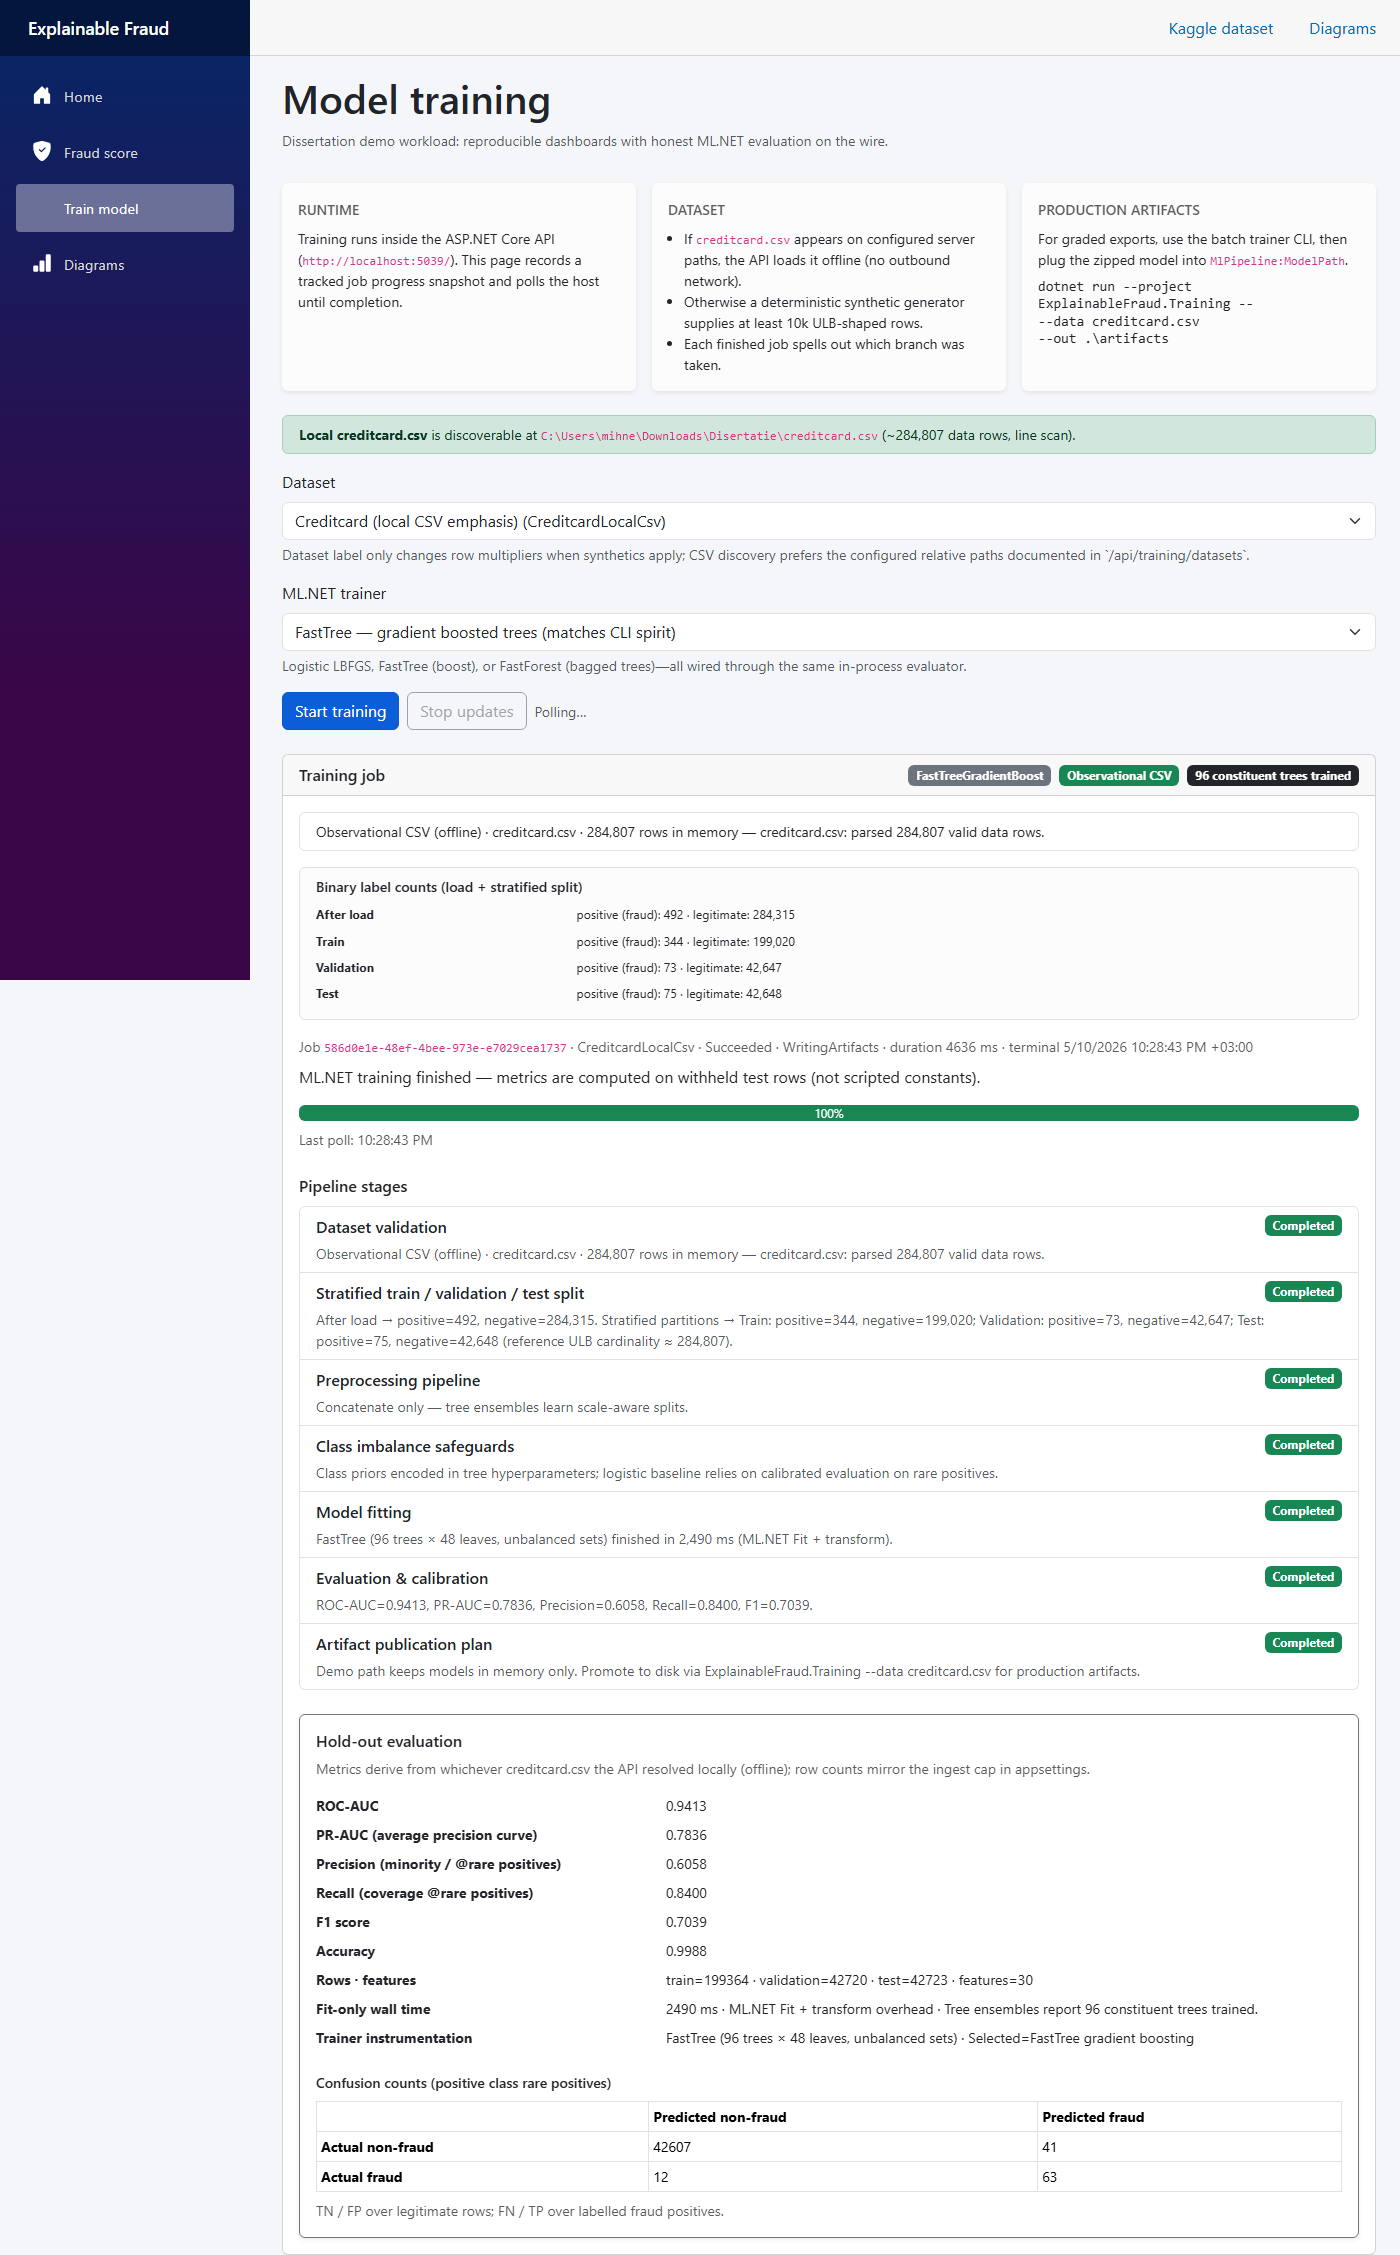
\includegraphics[width=0.82\linewidth,height=0.62\textheight,keepaspectratio]{figures/ui-training-success.png}
\caption{Successful CSV-backed FastTree training run on \texttt{/training}: observational data-source banner (full \texttt{creditcard.csv}, $\approx 284{.}8\mathrm{k}$ rows), stratified-stage transcript with evaluator line, and metric card mirroring Chapter~5.}
\label{fig:ui-training-success}
\end{figure}

\paragraph{Regression tests as release gate.}
The \texttt{Explainable\allowbreak Fraud.\allowbreak UnitTests} project couples heuristic scoring checks with training orchestration suites: neural-placeholder rejection, simulation toggles, FastTree success on deterministic synthetics (metric ranges, confusion mass positivity, stage cardinality, data-source labelling), timeline-only divergence, and per-family \texttt{InProcess\allowbreak Creditcard\allowbreak StyleTrainer} smoke fits. Maintainers should run \texttt{dotnet test} before claiming demo stability; thesis discussions may cite passing test matrices tied to defended commits.

\paragraph{Explainability coupling after training.}
\texttt{/fraud} explanations remain bound to whichever serialised model \texttt{IFraud\allowbreak ScoringService} loads. Training dashboards therefore explore candidate estimators disjoint from examiner-facing payloads until zipped artefacts and metadata migrate into configured model directories; scholarly prose must keep that firewall explicit when linking RQ2/RQ3 arguments to artefacts users actually touched.

\section{Architectural synopsis of the user journey}
Condensed retrospective: configuration binds HTTP clients and ML services; Razor components translate domain responses into actionable cards while preserving discriminator--explainer separation consistent with Chapter~3. The screenshots in Figures~\ref{fig:ui-fraud-form} and~\ref{fig:ui-fraud-scored} freeze this choreography for archival evidence within the dissertation.

\begin{figure}[htbp]
\centering
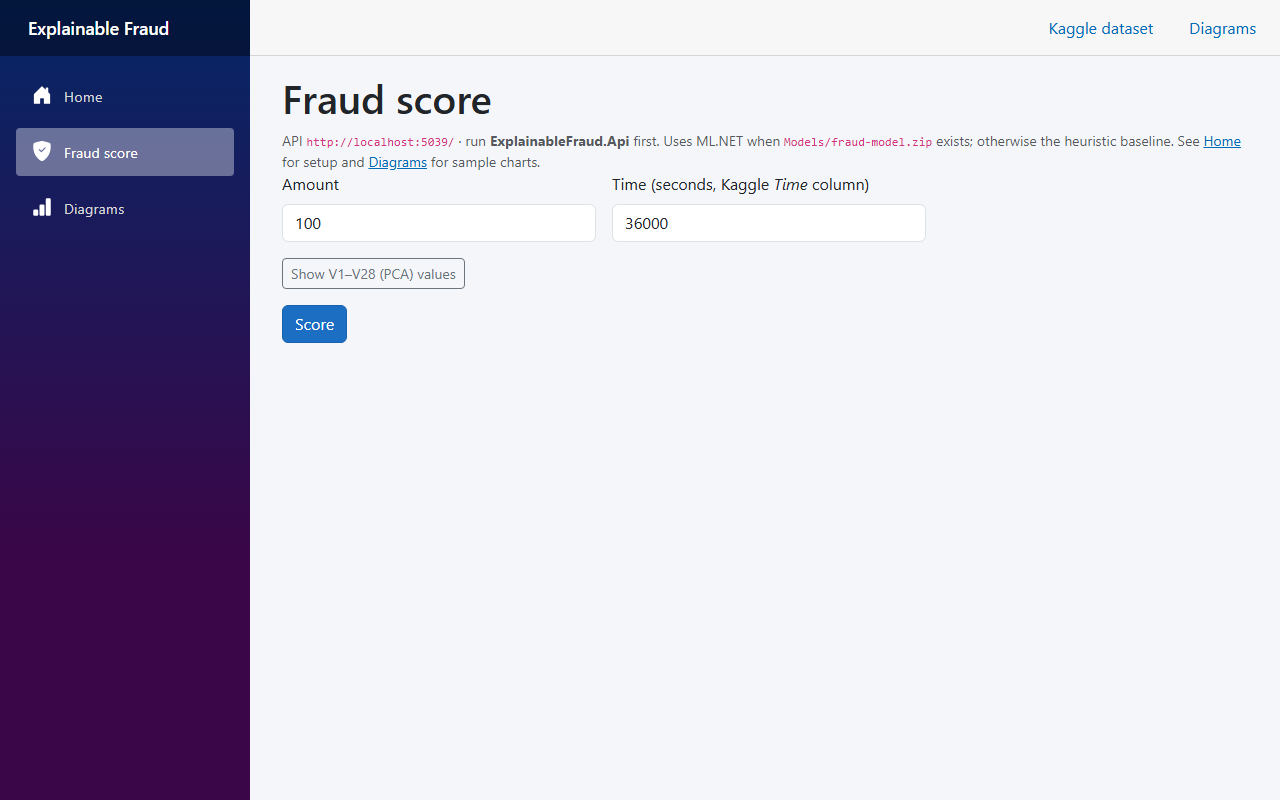
\includegraphics[width=0.92\linewidth]{figures/ui-fraud-form.png}
\caption{Blazor fraud scoring form (\texttt{/fraud}): input fields for amount and time, optional PCA vector, and contextual help linking documentation routes.}
\label{fig:ui-fraud-form}
\end{figure}

\begin{figure}[htbp]
\centering
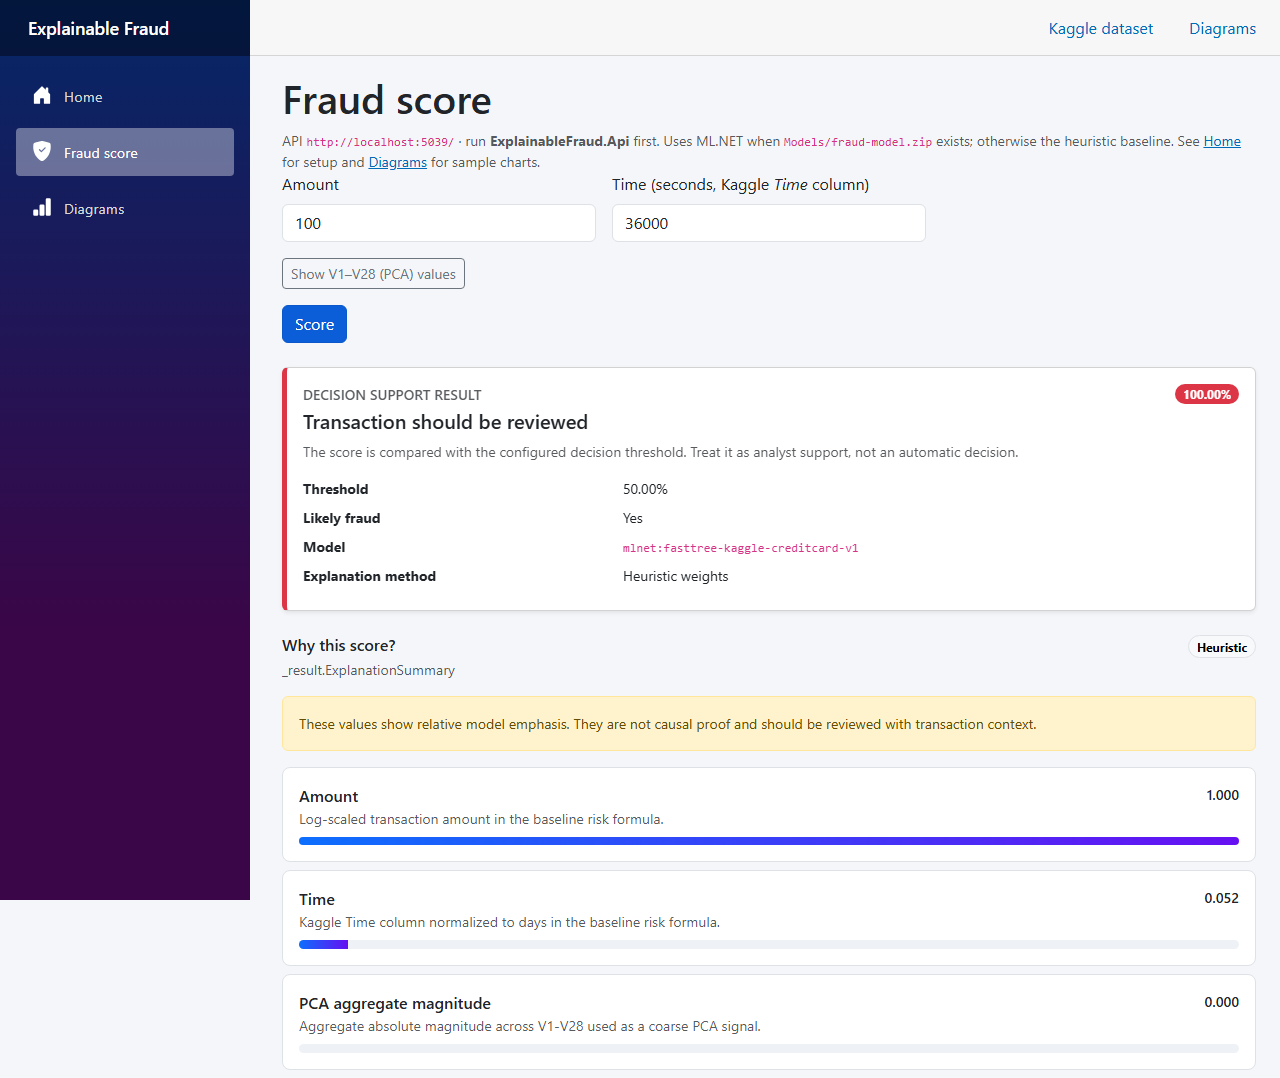
\includegraphics[width=0.92\linewidth]{figures/ui-fraud-scored.png}
\caption{Scored view: decision support card (threshold comparison, model version, explanation method), optional validation metrics, and ranked feature contributions.}
\label{fig:ui-fraud-scored}
\end{figure}

\section{Architecture and Dependency Injection}
Projects follow a pragmatic clean-architecture split, keeping JSON contracts and domain types separate from ML runtime code. Figure~\ref{fig:clean-arch-layers} summarises layer responsibilities; Figure~\ref{fig:request-flow} traces one scoring request across process boundaries.

\begin{figure}[htbp]
\centering
\resizebox{\linewidth}{!}{% Layer alignment of the ExplainableFraud solution (conceptual).
% Designed to fit \linewidth with \resizebox in the host document, but kept
% reasonably compact so the rendered figure stays legible.
\begin{tikzpicture}[
  font=\small,
  layer/.style={draw, rounded corners=3pt, text width=10.5cm,
                minimum height=0.95cm, align=left, inner xsep=8pt, inner ysep=4pt},
  side/.style={draw, dashed, rounded corners=3pt, text width=4.6cm,
               align=center, inner xsep=6pt, inner ysep=4pt, fill=gray!6},
  >=Latex
]
  \node[layer, fill=red!6] (web)
    {\textbf{Presentation} --- \texttt{ExplainableFraud.Web}\\
     (Blazor, \texttt{IFraudScoringApi}, shared Razor components)};
  \node[layer, fill=yellow!15, below=0.30cm of web] (api)
    {\textbf{HTTP API} --- \texttt{ExplainableFraud.Api}\\
     (controllers, serialisation, CORS to the Blazor origin)};
  \node[layer, fill=green!7, below=0.30cm of api] (contracts)
    {\textbf{Contracts + domain types} --- \texttt{ExplainableFraud.Contracts}
     (JSON DTOs), \texttt{ExplainableFraud.Domain} (\texttt{TransactionFeatures})};
  \node[layer, fill=cyan!8, below=0.30cm of contracts] (app)
    {\textbf{Application} --- \texttt{ExplainableFraud.Application}
     (\texttt{IFraudScoringService}, \texttt{TransactionMapper})};
  \node[layer, fill=blue!10, below=0.30cm of app] (infra)
    {\textbf{Infrastructure} --- \texttt{ExplainableFraud.Infrastructure}
     (\texttt{MlNetFraudScoringService}, \texttt{HeuristicFraudScoringService},
      model path options)};

  \node[side, right=0.6cm of contracts] (training)
    {\scriptsize Training CLI\\\texttt{ExplainableFraud.Training}\\
     (writes model zip + metadata)};
  \draw[->, thick] (contracts.east) -- (training.west);
\end{tikzpicture}
}
\caption{Solution layering: Blazor UI and ASP.NET Core API are separate host processes; contracts and domain types sit between HTTP boundaries and application abstractions; infrastructure loads ML.NET pipelines or falls back to a deterministic heuristic when no model file is configured or found.}
\label{fig:clean-arch-layers}
\end{figure}

\begin{figure}[htbp]
\centering
\resizebox{\linewidth}{!}{% TikZ figure: Blazor UI -> HTTP -> API -> application service -> scoring -> DTO response.
% Wrapped with \resizebox{\linewidth}{!}{...} at the call site for safe width fit.
\begin{tikzpicture}[
  font=\small,
  >=Latex,
  box/.style={draw, rounded corners=2pt, align=center, inner sep=5pt,
              minimum width=3.4cm, minimum height=1.05cm},
  arrow/.style={->, thick}
]
  \node[box, fill=blue!8] (ui) {Blazor UI\\\textit{(Interactive Server)}};
  \node[box, fill=blue!8, right=1.1cm of ui] (http)
    {\texttt{HttpClient}\\\texttt{POST}\\\texttt{api/fraud/}\texttt{score}};
  \node[box, fill=orange!10, right=1.1cm of http] (api)
    {ASP.NET Core\\\textit{FraudController}};
  \node[box, fill=green!8, below=1.2cm of api] (app)
    {\texttt{IFraud-}\\\texttt{ScoringService}\\\textit{Application}};
  \node[box, fill=violet!8, right=1.1cm of app] (infra)
    {ML.NET or\\heuristic engine};
  \node[box, fill=gray!12, below=0.9cm of app] (dto)
    {\texttt{FraudScore-}\\\texttt{Response}\\JSON to UI};

  \draw[arrow] (ui) -- node[above, sloped, font=\scriptsize] {configured \texttt{ApiBaseUrl}} (http);
  \draw[arrow] (http) -- (api);
  \draw[arrow] (api) -- node[left, font=\scriptsize, xshift=-2pt] {map DTO $\rightarrow$ domain} (app);
  \draw[arrow] (app) -- node[above, font=\scriptsize] {predict + explain} (infra);
  \draw[arrow] (infra) |- (dto);
  \draw[arrow] (dto) -| (ui);
\end{tikzpicture}
}
\caption{End-to-end request flow from interactive UI to JSON response. The API maps contracts to domain features, delegates to \texttt{IFraud\allowbreak ScoringService}, and returns a \texttt{Fraud\allowbreak Score\allowbreak Response} consumed by Razor components.}
\label{fig:request-flow}
\end{figure}

Registration occurs in \texttt{Program.cs} files: the API calls \texttt{AddInfrastructure(\allowbreak configuration)} which binds \texttt{Ml\allowbreak Pipeline\allowbreak Options} (model path, threshold, labels) and resolves \texttt{IFraud\allowbreak ScoringService} as a singleton---either \texttt{MlNet\allowbreak Fraud\allowbreak ScoringService} when the zip exists, or \texttt{Heuristic\allowbreak Fraud\allowbreak ScoringService} otherwise (useful for CI or first-run demos). The web host registers a typed \texttt{HttpClient} and \texttt{IFraud\allowbreak ScoringApi}.

\section{Scoring and Explainability Interaction}
\label{sec:scoring-explainability}
At inference, \texttt{MlNet\allowbreak Fraud\allowbreak ScoringService} runs the ML.NET \texttt{Prediction\allowbreak Engine}, clamps the predicted probability, and constructs explanations by combining globally stored feature importance with per-feature deviation from training means (z-style scaling). Contributions are sorted for presentation and tagged with \texttt{Explanation\allowbreak Method.\allowbreak Metadata\allowbreak Weighted\allowbreak Deviation} to signal that this is an approximate, audit-oriented emphasis mask---not a LIME or SHAP oracle. When no trained pipeline is available, the heuristic service emits a transparent baseline so the UI stack remains testable.

This design supports RQ2 and RQ3 directly: the UI surfaces the declared explanation method and keeps narrative disclaimers adjacent to numeric scores; model metadata can attach offline validation metrics, reinforcing honest reporting when probabilities are displayed alongside qualitative rationales.

\section{HTTP Surface and Data Transfer Objects}
The public HTTP surface is intentionally narrow: a single scoring endpoint documented interactively via Swagger (Figure~\ref{fig:api-swagger}).

\begin{figure}[htbp]
\centering
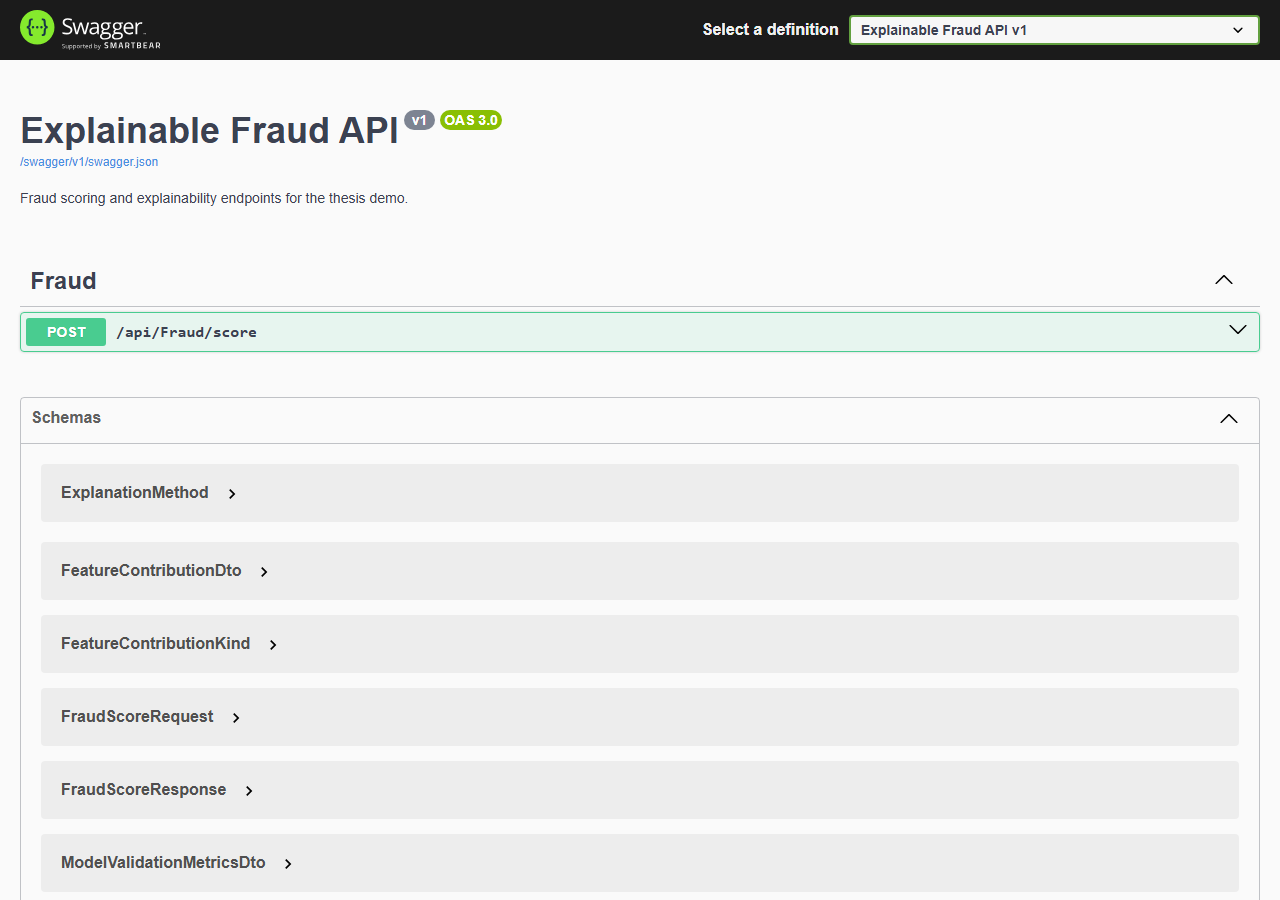
\includegraphics[width=0.95\linewidth]{figures/api-swagger.png}
\caption{OpenAPI/Swagger UI for the development API (\texttt{/swagger}), listing fraud scoring plus training routes (\texttt{/api/training/datasets}, \texttt{/api/training/jobs}, \texttt{/api/training/jobs/\{jobId\}}) and shared contract types.}
\label{fig:api-swagger}
\end{figure}

\noindent
Listing~\ref{lst:fraud-controller} shows how the controller stays thin: validate body implicitly via ASP.NET Core, map to \texttt{Transaction\allowbreak Features}, delegate scoring, return \texttt{Fraud\allowbreak Score\allowbreak Response}. Listing~\ref{lst:fraud-client} shows the symmetrical client call issued by the web project.

\lstinputlisting[
  float=htbp,
  language=CSharp,
  style=csharpsnippet,
  firstline=8,
  lastline=22,
  caption={API adapter: \texttt{FraudController} maps DTOs via \texttt{TransactionMapper} and returns a contract response (\texttt{ExplainableFraud.Api/\allowbreak Controllers/\allowbreak FraudController.cs}).},
  label={lst:fraud-controller}
]{ExplainableFraud/src/ExplainableFraud.Api/Controllers/FraudController.cs}

\lstinputlisting[
  float=htbp,
  language=CSharp,
  style=csharpsnippet,
  firstline=6,
  lastline=21,
  caption={Blazor client wrapper: JSON POST to \texttt{api/fraud/score} with deserialization to \texttt{Fraud\allowbreak Score\allowbreak Response} (\texttt{ExplainableFraud.Web/\allowbreak Services/\allowbreak FraudScoringApi.cs}).},
  label={lst:fraud-client}
]{ExplainableFraud/src/ExplainableFraud.Web/Services/FraudScoringApi.cs}

DTO shape highlights:
\begin{itemize}
    \item \textbf{Request:} \texttt{Amount}, \texttt{Time}, optional \texttt{Principal\allowbreak Components} (length $\leq 28$, validated in \texttt{Fraud\allowbreak Score\allowbreak Request}).
    \item \textbf{Response:} fraud probability, decision threshold, Boolean likely-fraud flag, explanation method enum, contribution list (\texttt{Feature\allowbreak ContributionDto}), model version string, optional validation metrics from training exports.
\end{itemize}

\section{Reusable User Interface Components}
Shared Razor components separate presentation concerns: \texttt{RiskSummaryCard} emphasises threshold comparison and reframes output as decision support (not autonomous adjudication); \texttt{Explanation\allowbreak Contributions} renders ranked evidence; \texttt{Validation\allowbreak MetricsCard} surfaces PR-AUC and F$_1$ when embedded in model metadata. This modular structure keeps the main page focused on data entry while ensuring consistent visual language for RQ-motivated messaging (threshold literacy, explanation caveats).

\section{Relation to Empirical Chapter}
The empirical investigation chapter continues with offline metrics tables and interpretive critique; the present chapter supplies the deployment-shaped lens---how those metrics could be reflected in UI metadata when models are versioned with their evaluation JSON. Readers should treat screenshots and flows here as implementation evidence accompanying, not replacing, the statistical claims that follow.

\section{Scripted clients and API parity with analyst workflows}
While the Razor interface targets human operators, reproducible scholarship routinely demands scripted replays devoid of transient UI interactions. Swagger (\texttt{/swagger}) documents request JSON schemata and enables teams to replay identical payloads with command-line tooling or integration tests (\texttt{curl}, \texttt{REST Client}, bespoke \texttt{xUnit} suites). Maintain parity principles: scripted calls should reference the same \texttt{POST} routes and contract types as interactive sessions so that divergence between manual demos and archived logs never masquerades as model drift.

\textbf{Correlation with automated evaluation.} When Chapter~5 finalises thresholds, scripted smoke tests might assert deterministic ordering (\emph{e.g.}, monotonicity sanity checks against synthetic vectors) whereas statistical tests occupy offline notebooks---the ExplainableFraud stack intentionally keeps those concerns separate lest lightweight CI degrade into stochastic acceptance gates susceptible to flaky seeds. Training orchestration adds complementary \texttt{xUnit} coverage (Section~\ref{sec:training-surface}) asserting that exploratory ML.NET jobs either surface evaluator-backed metrics or remain explicitly labelled simulations.

\textbf{Synthetic payloads for teaching.} Instructors composing classroom scenarios can initialise extreme amount/time pairs to demonstrate score saturation, illustrating how nonlinear tree ensembles clip contributions compared with linear likelihood models. Companion warnings in UI copy remind novices not to extrapolate behavioural conclusions from exploratory stress inputs.

\section{Regression testing, configuration drift, and academic reproducibility}
Configuration objects (\texttt{Ml\allowbreak Pipeline\allowbreak Options}; \texttt{TrainingJobs:\allowbreak Simulation}) unify model filenames, thresholds, ingestion probes, simulated dataset sizing, trainer toggles, and human-readable identifiers. Scholars packaging dissertation supplements should freeze these parameters alongside PDF outputs: hash or checksum artefacts in repository readmes assists examiners validating that submitted binaries align with authored narrative. Automated harnesses activating \texttt{Heuristic\allowbreak Fraud\allowbreak Scoring\allowbreak Service} guarantee build success even absent proprietary model zips---a pragmatic concession for anonymous review---but manuscripts must annotate whenever screenshots stem from calibrated pipelines versus heuristics; likewise, narrated training dashboards require synchronized disclosure of CSV-backed versus synthetic ingestion together with contemporaneous passing \texttt{dotnet test} transcripts.

Environment drift (\texttt{.NET} feature bands, NuGet minors, deterministic ML.NET RNG policies) subtly perturbs floats; versioning lockfiles strengthens replication even if bitwise equality remains elusive across CPU generations. Where exact reproduction fails, documenting expected tolerance bands on $\hat{y}$ preserves intellectual honesty consonant with RQ3's calibration cautions.

\section{Reproducing Screenshots and Diagrams}
Screenshots in Figures~\ref{fig:ui-fraud-form}--\ref{fig:api-swagger} were captured with Playwright from local development URLs (Blazor HTTP profile on port~5246; API Swagger on port~5039). Launch commands use the HTTP launch profiles bundled with each project; the web configuration must point \texttt{ApiBaseUrl} at the running API. The script \path{scripts/capture-fraud-result.mjs} regenerates the post-score figure after \texttt{npm install} at the repository root.

\noindent
Figure~\ref{fig:ui-training-success} archives a regenerated Playwright capture once \texttt{creditcard.csv} resolves at the repository root (\path{figures/ui-training-success.png}). Scripted replay uses \texttt{node scripts/\allowbreak capture-training-success.mjs} after launching both ASP.NET profiles (Blazor~\texttt{:5246}, API~\texttt{:5039}).
